%%% Local Variables:
%%% TeX-master: "AbilityMaster"
%%% End:%%% Local Variables:
%%% TeX-master: "master"
%%% End:

\chapter{Potentive entailment --- Attribution and Witnessing}
\label{cha:potent-infer-attr}

\begin{note}[Overview]
  In this chapter focuses on understanding potentive entailment, potentive entailment with respect to (specific) abilities, and how potentive entailment with respect to (specific) abilities is used in the cases of interest.
\end{note}

\begin{note}[Plan for chapter]
  The plan for the chapter is as follows:
  \begin{itemize}
  \item Potentive entailment.
  \item Two ways in which potentive entailment may be used --- \AR{} and \WR{}.
  \item Differences between \AR{} and \WR{}.
  \item (Possibly) further notes on \WR{}.
  \end{itemize}
\end{note}

\begin{note}[First part plan]
  Start with potentive entailment.
  This section will serve two purposes.
  First, clarify potentive entailment.
  Second, establish that potentive entailment does not require ability.

  Second is important as agent does not necessarily need to rely on ability attribution.
  In short, consequent follows from event, rather than predicate.
  Argue that the relevant use of ability may be treated as functionally analogous to an (existential) event quantifier.

  Not to say ability is not important.
  May be required in order for potential event to be true.
  However, backgrounded.
  Entailment follows from potential, and potential may require attribution of ability, but only in so far as the antecedent needs to hold.

  This will provide the setup for the two ways potentive entailment may be used in scenarios of interest.
\end{note}

\begin{note}[Second part plan]
  Potentive entailment.
  Simply provides information.
  Distinct from establishing a support relation.

  Two ways in which potentive entailment may be used from understanding different support relations made available by entailment.
  Argue that there is no plausible third option, on the basis of potentive entailment (though this does not rule out independent sources).
\end{note}

\begin{note}[Third part plan]
  Potentive entailment.
  Differences in support.

  Potentive entailment is going to hold independent of support.
  Question whether there is further difference, or whether \AR{} and \WR{} come as a pair.

  So, look for ways to distinguish \AR{} and \WR{} with respect to support.
  Argue that these depend on further commitments that we may remain neutral on.
\end{note}

\begin{note}[Wrapping up]
  So, this chapter concludes with a clear understanding of how potentive entailment relates to main argument.
\end{note}

\begin{note}[Extras]
  Appendix to the chapter contains further remarks on potentive entailment, as it seems that this isn't something that's been discussed too much.
\end{note}


\section{Potentive entailment}
\label{sec:potentive-entailment}

\subsection{The entailment}
\label{sec:entailment}

\begin{note}[Potentive entailment]
  The canonical form of potentive entailment is:
  \begin{enumerate}
  \item In order for there to be potential for some event \(e\) to be witnessed, \(\psi\) must (already) be the case.
  \end{enumerate}
  Intuitively, there is potential for some event \(e\) to be witnessed if there are preconditions for witnessing that must been met, and the potentive entailment identifies \(\psi\) as some such precondition that has been met.

  Term this `potentive entailment' as consequent of the entailment follows from the `potential' construct of the antecedent.
  
  For example, there is potential for Smith to travel to London in time for tomorrows meeting.
  So, there is an aeroplane set to depart no later than midnight tonight for which Smith may purchase a ticket, and so on.
  
  This is `local' entailment.
  It does not look for necessary conditions for an event.
  For example, private jet.
  Given the way things are, no private jet.

  So, hard to determine whether a potentive entailment holds in general.
  May be some exception.

  For present purposes, there is potential for some event to be witnessed.

  Specially, the events of interest are an agent reasoning from some premises to a conclusion.

  \begin{enumerate}
  \item\label{PE:ability:event} As there to be potential for an event of S proving \(\phi\) to be witnessed, \(\psi\) must (already) be the case.
  \end{enumerate}

  Example.

  Finally, change of focus to the agent rather than the potential event.
  Potential for an event of \dots to be witnessed, rewrites to S has the ability to \dots

  \begin{enumerate}
  \item\label{PE:ability:agent} S has the (specific) ability to V that \(\phi\), so \(\psi\) must (already) be the case.
  \end{enumerate}

  Remains an instance of potentive entailment.

  Given that~\ref{PE:ability:event} and~\ref{PE:ability:agent} we avoid the need for an understanding of ability.
  Some worries about what it is for there to be a potential event.
  Suitable analysis may depend on ability, or perhaps ability is analysed in terms of potential events.

  In short, while~\ref{PE:ability:agent} is natural, and our preferred statement, \ref{PE:ability:event} is equivalent.
  Therefore, we will understand the use of potentive entailments involving ability in terms of potential events, rather than on the basis of any particular understanding of ability.

  What matters is the event, and what must be the case in order for the event to be witnessed.

  Important thing to stress is that consequent does not necessarily follow from agent possessing ability.

  Still some differences, deal with these after examples.
\end{note}

\begin{note}[Examples]
  Simple instances of the potentive entailment involve factive verbs, in which the relevant fact holds independently of whether the verb is witnessed.
  \begin{itemize}
  \item Sam has the ability to show that \(19\) is a prime number.
  \item Taylor has the ability to derive Transposition.
  \item Jesse has the ability to \dots
  \end{itemize}

  Note also that the verb does not need to involve some reasoning.
  \begin{itemize}
  \item Corey has the ability to see there is a zebra in the pen.
  \item X has the ability to hear that there is a waterfall nearby.
  \end{itemize}
\end{note}

\begin{note}[Breaking things down]
  An instance of potentive entailment has an antecedent and consequent.
  As may be seen from the examples provided, there are no particular constraints on the consequent of a potentive entailment.
  The antecedent of potentive entailments of interest, however, have two main components:
  \begin{itemize}
  \item\label{pe:part:event} An event.
  \item\label{pe:part:modal} A `potentive' modal applied to the event
  \end{itemize}
  The event in turn has three important components:
  \begin{enumerate}
  \item\label{pe:part:agent} An agent.
  \item\label{pe:part:verb} A verb describing some action performed by the agent.
  \item\label{pe:part:result} Some result of a successful performance of the action described by the verb.
  \end{enumerate}

  Gave a gloss of potentive entailment.

  Key observation 1.
  Possible consequents are determined by the event, rather than the modal.
  Obtain consequent because of the modal.

  So, each of the examples, we obtain the same entailment on the assumption that the event described has happened.

  Contrast.
  Potential for \(e_{1}\) and potential for \(e_{2}\), so potential for \(e_{3}\).
  E.g.\ conjunction introduction.

  In other words, the consequent does not hold because the event is a \emph{potential} event.
  Or, that this is `epistemic'.

  Well, consequent because the event of the antecedent requires the consequent.

  So, that the potential provides a way to get the consequent prior to the event happening.
  No instance of potentive entailment where the consequent follows because the event is potential.
  This is not to deny that there are cases in which entailment relies on potential.

  So, here explaining why the work is done primarily by the verb.
  Might think that using `discovers' is a counterexample.
  Only possible because the action involved is for the moment potential.
  However, the verb itself does the work here.
  Get the consequent that the agent hasn't done the reasoning, but understanding this as simply shifting temporal index.

  So, the important of this key observation is that we further reduce interest in ability.
  We've seen that alternative modal may be used.
  And now that the modal is of secondary importance.
  
  
  
  Two candidates for the antecedent.
\begin{quote}
  \begin{enumerate}
  \item There is a potential event in which \emph{S} \emph{V}s that \(\phi\).
  \item \emph{S} has the ability to \emph{V} that \(\phi\).
  \end{enumerate}
  \end{quote}
\end{note}

\begin{note}[Two important instances of potentive inference]
  Restate information.
  Apply potentive inference.

  Two important instances of potentive inference
  \begin{enumerate}
  \item Conclusion is the case.
  \item Support for premises.
  \end{enumerate}
\end{note}

\subsubsection{Hum}
\label{sec:hum}

\begin{note}[Potentive]
  The potentive is straightforward to analyse.

  Fairly clear understanding of event semantics.

  Here, existential quantification over events is replaced by a modal.

  This requires some non-standard existential, but we're not too interested in providing an analysis suitable for semantics.
\end{note}


\begin{note}[Understanding potentive entailment]
  The key parts of the entailment are the relation between ability and the verb.

  Certain things must be true in order for the verb.
  These are the things which are obtained by the potentive entailment.

  In the case of reasoning, note that there must be premises from which the agent works from.
\end{note}



\begin{note}[Ability]
  Our understanding of ability is basically the same as potentive.

  Ability functions as an equivalent quantifier.

  Specific reading of ability.
  \textcite{Hackl:1998tt} distinguishes:
  {
    \small
    \begin{enumerate}
    \item John is able be a tall (in view of the evidence available).\hfill \emph{epistemic}
    \item John is able to listen to punk rock.\hfill \emph{deontic: ``allowed-to-do''}
    \item John is able to be married, according to the law.\hfill \emph{deontic: ``allowed-to-be''}
    \item John is able to jump higher than Bill.\hfill \emph{ability}
    \item John is able to see Mary from where he is standing.\hfill \emph{opportunity}
    \end{enumerate}
  }
  Only the last two readings seems natural, but all work if `able to' is read as `can'.

  We're interested in what \citeauthor{Hackl:1998tt} terms `opportunity'.
\end{note}

\begin{note}[Avoid ability?]
  A simple corollary of the above observations potentive entailment does not require ability.

  If it is possible to provide information about potential event of reasoning without attributing ability, then we don't need to speak of ability at all, perhaps with the exception of generating intuitive scenarios.

  May wonder how important ability is.

  Difficult case.
  Go for externalism, and co-reference.
  State a conclusion, but the agent would not reason to the conclusion under that description.

  There's a potential event, but it isn't clear that the agent has the ability.

  Doubt this is possible, as agent needs to do something.
  And, ability this seems sufficient for an ability statement.
  So, continue to work with ability.
\end{note}

\begin{note}[Some formal stuff]
  \[(\text{Able}(s,e) \land (V(e) \land \text{agent} = s \land \text{result}(e) = \phi))\]
  There is some event \(e\), such that \emph{s} is able to bring about, and \(e\) consists of \emph{s} \emph{V}ing with the result that \(\phi\).

  The quantification here is somewhat familiar to Lewis' counterpart theory.

  Understand ability as relating the agent directly to an event.
  Alternative it to take a truth value.
  \((\text{Able}(s,\exists (V(e) \land \text{agent} = s \land \text{result}(e) = \phi))\).

  Close to having a possible world with \(\phi\) and accessibility relation.
  Interpret the non-standard existential in this way, if it helps.
  There is some possible world and some event in that world, such that the agent at the world of evaluation is able to perform the event witnessed at the possible world.

  In both cases, it's the role of the event.

  \begin{figure}[h]
    \begin{subfigure}{.5\textwidth}
      \centering
      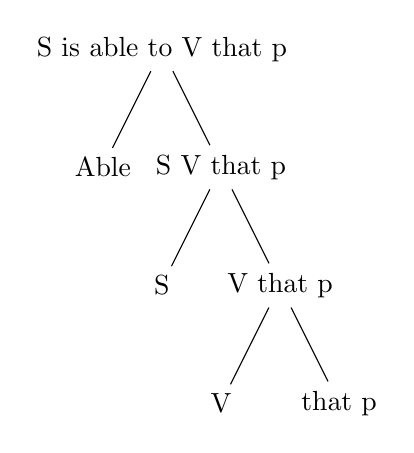
\begin{tikzpicture}[
        ]
        \node{S is able to V that p}
        child {node {Able}}
        child {node {S V that p}
          child {node {S}}
          child {node {V that p}
            child {node {V}
            }
            child {node {that p}
            }
          }
        };
      \end{tikzpicture}
    \end{subfigure}
    %
    \begin{subfigure}{.5\textwidth}
      \centering
      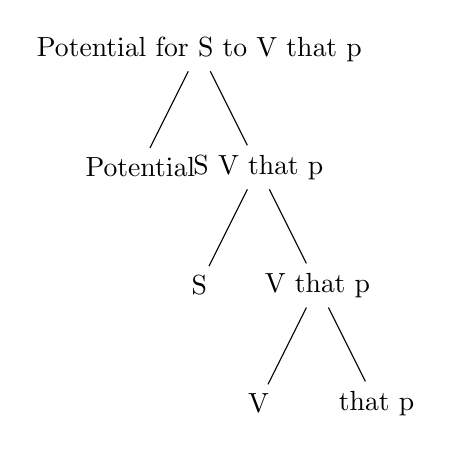
\begin{tikzpicture}[
        ]
        \node{Potential for S to V that p}
        child {node {Potential}}
        child {node {S V that p}
          child {node {S}}
          child {node {V that p}
            child {node {V}
            }
            child {node {that p}
            }
          }
        };
      \end{tikzpicture}
    \end{subfigure}
  \end{figure}
  Suggestion here is that there's really nothing too interesting.
  In both cases it seems possible to have a complete description of the witnessing event prior to the introduction of a modal.
  Only complexity involved is projecting agent from event in order to apply ability.
\end{note}

\begin{note}[The entailment]
  Take some arbitrary witnessing event.
  If \(\psi\) follows from the (arbitrary) witnessing event, then we have an instance of the potentive entailment.

  Pretty much the same as reasoning with existentials.
\end{note}

\begin{note}[Expanding the event]
  The description of the witnessing event given is minimal.
  Still, simply add in more detail as desired.
\end{note}


\begin{note}[Observation in terms of prop/dox]
  One way to view this is that if the agent has information, then the agent may infer that they have propositional support for the conclusion which may be turned in to doxastic support.
\end{note}

\begin{note}[Specific abilities]
  Applies to specific abilities, as the entailment appeals to a witnessing event.
  Analogue holds with respect to general abilities.

  General example:
  \begin{itemize}
  \item Sam has the ability to reason with the rules of chess.
  \end{itemize}
  Infer that there is a body of rules governing chess.
  If there are no rules governing chess, then the agent does not have the ability to reason with those (non-existing) rules.

  Not an instance of the potentive entailment, as this doesn't follow from what is required from a witnessing event.

  Similarly, it may be that there is an entailment from general to specific.
  \begin{itemize}
  \item If general, then specific.
  \end{itemize}
  For example, understand the general ability distributively.
  Again, not an instance of the potentive entailment, as this doesn't follow from what is required from a witnessing event.
\end{note}

\begin{note}[Paraphrasing (footnote)]
  Various paraphrases are available.
  \begin{itemize}
  \item Corey can see there is a zebra in the pen.
  \end{itemize}
  `Can' introduces the complexity that the agent may be witnessing.
  For example, we observe an excited look appear on Corey's face as they look into the pen.
  `Ah, Corey can see a zebra in the pen.'
  Corey isn't exited because they have the ability to see a zebra in the pen, rather Corey is excited because they are seeing a zebra.
\end{note}

\subsection{Our interest in potentive entailment}
\label{sec:our-inter-potent}

\begin{note}[Restriction on instances of potentive entailment]
  We're interested in certain examples as the agent has all of the resources required, so to speak.

  To illustrate, place the reasoning examples behind a conditional.
  \begin{itemize}
  \item If you teach Sam \dots [factoring method], then Sam will have the ability to show that \(19\) is a prime number.
  \end{itemize}
  Intuitively, this is the result of assuming that some additional property holds of the agent.
  Hence, \(\alpha(s) \rightarrow \dots\).
  For, \(\alpha(s)\) will allow the attribution of ability to be true.
\end{note}

\begin{note}[Reasoning and premises]
  Important to note is that in cases of reasoning, the potentive entailment may be applied to obtain the availability of premises.

  The difference is the role of these premises.
\end{note}

\begin{note}[Two instances of potentive entailment]
  We get premises and conclusion.

  Here, the important thing is that if the agent doesn't already have the basics, then something further would need to be the case for there to be a potential event.

  Admittedly, there is no clear line.
  For, there are ways to expand the event.

  Example, lighting a match.
  Have match and matchbox in hand.
  Have matchbox.
  Matchbox is in a draw.
  Etc.

  Resolved by placing constraints on the event.
\end{note}

\begin{note}[Moving on to a more detailed understanding]
  How exactly the event works.
\end{note}

\section{\AR{} and \WR{}}
\label{sec:ar-wr}

\begin{note}[Overview]
  Interest is in how potentive entailment is used.

  A clearer understanding of \AR{} and \WR{}.

  The significant difference is with reasoning.
  \AR{} uses (a variation of) the potentive entailment to obtain support.
  \WR{} uses information obtained by the potentive entailment to obtain support.
\end{note}

\subsection{Entailment and support}
\label{sec:entailment-support}

\begin{note}[Overview]
  The previous section provided an overview of potentive entailment.
  The following sections will explore the use of potentive entailment when an agent reasons with information that they have the ability to reason to some conclusion.
  The present section argues a premise that will be used in the following sections.

  \begin{enumerate}
  \item\label{PE+S:epistemic} Entailment is `epistemic'
  \item\label{PE+S:diff-support} Instances in which information about an entailment allows an agent to establish a relation of support between some premise and conclusion, where the premise and conclusion may be distinct from the antecedent and consequence of the entailment.
  \end{enumerate}
  The upshot of~\ref{PE+S:diff-support} is that it is, at least conceptually, possible that any agent may recognise that a potentive entailment holds, and uses the entailment to establish support.
\end{note}

\begin{note}[Epistemic]
  The entailment is epistemic.
  Meaning, information of antecedent is sufficient to establish consequent.
  It is not the case that the consequent holds because the antecedent holds.
\end{note}



\begin{note}[Quick test]
  Potential \(e\) is the reason why \(\psi\).
  \(\psi\) is the reason why there is potential \(e\).

  Some good instances and some bad.

  Bad is the flight example.
  These are, in the appropriate sense, preconditions.
  So, the relation of support is inverted.

  However, from epistemic perspective, things may go the other way.
\end{note}

\begin{note}[Tracks example]
  There are tracks \dots

  So, why provides support?

  Another is reading a clock.
\end{note}

\begin{note}[Translation]
  Someone says something false.
  Hold them to be a liar.

  Translation.
  A little murky.

  Still, develop a little more.
  Informer provides basics of translation.
  Now the agent has translated.
\end{note}

\begin{note}
  These are examples in which it seems, at least on the surface, plausible that information provided allows the agent to establish a support relation.
\end{note}

\begin{note}[Two premises so far]
  \begin{enumerate}
  \item Potentive entailment need not establish support.
  \item Instances in which information allows for distinct support relations.
  \end{enumerate}
\end{note}

\begin{note}[Okay with uRa]
  As an aside, these examples are compatible with \ref{denied-claim}.
  The issue is with what establishes support.
  \ref{denied-claim} only details `access', and in these examples the options for support seem accessible.
\end{note}

\subsection{Entailment, support, and the ability to reason}
\label{sec:enta-supp-abil}

\begin{note}[Ability to reason]
  The important thing to keep in mind is that if the agent has the ability, then the agent has propositional support, so to speak.
  This is not required for potentive entailment, which is far more general.
  However, we develop \AR{} and (in particular) \WR{} with this assumption in mind.
\end{note}

\begin{note}[\AR{} and \WR{}]
  Have conclusion obtained by potentive entailment.

  Support is traced from ability/potential.
  Support is traced from premise obtained by potentive entailment.
\end{note}

\begin{note}[Diagram]
  \begin{figure}[h]
  \begin{subfigure}{.5\textwidth}
    \centering
    \begin{tikzpicture}[
      ->,
      >=stealth',
      % auto,
      node distance=0cm, every text node part/.style={align=center},
      ]

      \node [] (c) at (0,0) {};
      \node [] (d) at (-3,0) {};
      \node [] (e) at (3,0) {};
      \node [] (f) at (0,-2.1) {};

      \node (1) at (0,-.1) {Ability};
      \node (2) at (0,-2) {Conclusion};

      \draw [->] (1.270) to [] node[left] {} (2.90);
    \end{tikzpicture}
    \caption{\AR{}}
    \label{fig:AR:support}
  \end{subfigure}
  % \hfill
  \begin{subfigure}{.5\textwidth}
    \centering
    \begin{tikzpicture}[
      ->,
      >=stealth',
  % auto,
      node distance=0cm, every text node part/.style={align=center},
      ]

      \node [] (c) at (0,0) {};
      \node [] (d) at (-3,0) {};
      \node [] (e) at (3,0) {};
      \node [] (f) at (0,-2.1) {};

      \node (premise) at (0,-.1) {Premise};
      \node (conclusion) at (0,-2) {Conclusion};

      \node (x) at (-2,-1.05) {Ability};
      \draw [->] (1.270) to node[left] (3) {} (2.90);

      \node (4) [left of=3, xshift=-2cm] {}; % {\(\exists f (f\Phi = \psi)\)};
      \draw [-{Circle[open]}, dashed] (x.0) to (premise);
      \draw [-{Circle[open]}, dashed] (x.0) to (conclusion);

    \end{tikzpicture}
    \caption{\WR{}}
    \label{fig:WR:support}
  \end{subfigure}
  \caption{Relations of support for \AR{} and \WR{}}
  \label{fig:ARandWR:support}
\end{figure}
\end{note}

\begin{note}[Examples of support relation]
  The interesting issue is the inaccessibility of the premises.
  However, there are other examples in which the same structure is present, but premises are accessible.
  
  Are there other instances of information being used in this way?

  Plausible that go from appearance to support.

  `You are looking at a dog'.

  Here, the agent can infer from testimony that the animal is a dog.
  On the other hand, the agent can take the information to establish a support relation.
  So, visual perception support that the animal is a dog.

  Or, a little better.
  These are coyote tracks.
  Then, different ways to support presence of coyote.
  One is the information provided.
  The other is the tracks.
\end{note}

\begin{note}[The event]
  Two ways for the potentive entailment to function.
  Both \AR{} and \WR{} focus on the witnessing event.

  \emph{V}ing that \(\phi\).
  \begin{itemize}
  \item \(\phi\) must be the case in order for the agent to \emph{V} that \(\phi\).
  \item In order for the agent to have the attribute \dots
  \item \(\phi\) is the result of the agent \emph{V}ing.
  \item As a result of witnessing the ability \dots
  \end{itemize}

  So, \AR{} doesn't consider the relevant witnessing, only what must be the case in order for there to be a witnessing event.
  By contrast, \WR{} focuses on guarantees about what transpires in the witnessing event.
\end{note}

\begin{note}[Multiple support relations]
  \AR{} and \WR{} differ in terms of support relations.
  This is the most important distinction for the broad argument of the thesis.

  Focus is on particular kind of ability: general to specific.

  Still, this provides us with at least three distinct support relations that may follow from an agent receiving information that they have the ability to reason to some conclusion, and prior to witnessing the ability.
  \begin{enumerate}
  \item \AR{}
  \item \WR{}
  \item Precondition of receiving information.
  \end{enumerate}
  In simple cases, all three may be available to an agent after receiving information.

  Question about how these interact.
  Support does not seem additive.
  
\end{note}

\subsection{\AR{}}
\label{sec:ar}



\subsection{\WR{}}
\label{sec:wr}

\begin{note}[Overview]
  In section~\ref{sec:ar-wr} we outlined the key distinction between \AR{} and \WR{} for the purpose of the overarching argument of this thesis.
  
  

  Understanding \WR{}.
\end{note}

\begin{note}[Work backwards for the event]
  Work backwards for the event
\end{note}

\begin{note}[How support works]
  In the case of reasoning, the result will be that the agent has information about premises.
  Here, it is important to note that the agent has `propositional' support for the premises, independent of the ability information.
  So, the agent does not need to appeal to the existence of the event as a premise in obtaining support for the conclusion.
  The only relevant support the agent has is the support for the premises.
\end{note}

\begin{note}[Similar applications of the basic idea]
  Introduce idea that this is something of a placeholder.
  Perhaps use the example from names with an as yet unidentified reference to provide additional motivation.

  The idea is similar in principle.
  There is someone out there in the world.
  Just as there is support that the agent may use.
  So, the remaining task is to fix the interpretation of the name.
  Likewise, the remaining task for the agent is to witness the relation of support.

  In both cases, establishing the additional stuff is useful.
  Foremost, resolves the possibility that the `future' may not be resolved.
  And, other minor benefits in terms of further information.
\end{note}



\subsection{Distinction between \AR{} and \WR{}}
\label{sec:dist-betw-ar}

\begin{note}[Overview]
  The important difference is what supports the conclusion.

  Here, we suggest that further differences depend on additional commitments.
\end{note}


\begin{note}[Key Issue]
  The key issue is whether the agent obtains support for all the relevant preconditions of witnessing the ability by witnessing.
  And, whatever follows from this, e.g.\ in terms of commitments and so on.

  If so, then anything that follows from \AR{} also follows from \WR{}.
  Conversely, as the agent does not obtain information about how the ability is witnessed, it seems what follows from \WR{} also follows from \AR{}.
\end{note}

\begin{note}[Interesting case]
  Interesting case to think about, in which the agent obtains support for what follows from witnessing, but intuitively not for some other precondition.
  \begin{itemize}
  \item Ability to reason to \(\phi\).
  \end{itemize}
  Entailment applies to \(\phi\).
  Entailment doesn't seem to apply to reasoning to \(\lnot\phi\) as mistaken.
\end{note}

Understanding of ability is such that there is always a potential witnessing event.

\ref{denied-claim} and~\ref{prem:ni} are universal claims.
\ref{prem:ab} is an existential claim.
\ref{denied-claim} and~\ref{prem:ni} clash in scenarios where the possibility captured in~\ref{prem:ab} is realised.

The collection of~\ref{denied-claim},~\ref{prem:ni}, and~\ref{prem:ab} is in tension.

There is an additional secondary premise:

\begin{note}[Two ways to understand ability and support]
\begin{enumerate}
\item\label{prem:ability} Two ways to obtain conclusion given ability.
  \begin{enumerate}
  \item Attribution.
  \item Witnessing.
  \end{enumerate}
\end{enumerate}

\ref{prem:ability} does not make a claim about any particular use of ability.
As a template, conceptually (or logically) coherent.
If there's a problem, then it's because there are further constraints on understanding of support.
\end{note}

\section{Miscellaneous}
\label{sec:misc}


\subsection{Additional observations}
\label{sec:addit-observ}

\begin{note}[Trouble with modals]
  We have sketched potentive entailment.
  However, noting the interaction between a modal and a verb.

  Understanding of why the entailment works has been left largely to intuition.

  The specifics of potentive entailment are not too important, so we may omit the detour.
  Still, even for those willing to make the detour it is not clear how long it would take, or where it would lead.

  Difficulty is seen by taking a straightforward treatment of the modals involved.

  `There is potential for' and `agent S has the (specific) ability to' are modals.

  Standard first pass at modals, via possible worlds and accessibility relations.

  Before continuing further, the presence of difficulty may be quickly noted by noting the similarities between potentive and actuality entailments.
  \textcite{Alxatib:2019wf} provides the following account of actuality entailments.
  \begin{quote}
    Actuality Entailments (AEs) are inferences from premises that appear to be modal, like (1a), but their content is that the modality is effectuated in the evaluation world --- (1b).

    \begin{enumerate}[label=(\arabic*)]
    \item
      \begin{enumerate}[label=\alph*.]
      \item Pierre a dû \hspace{26pt} prendre le \hspace{3.5pt} train \newline
        Pierre had.to.\textsc{pfv} take \hspace{14pt} the train\newline
        \hspace{-4pt} ‘Pierre had to take the train’
      \item \emph{Inference}: Pierre took the train.\nolinebreak
    \mbox{}\hfill\mbox{(\citeyear[701]{Alxatib:2019wf})}
      \end{enumerate}
    \end{enumerate}
  \end{quote}

  Note, the reading of `had' in (1a) is `unambiguously deontic' (\citeyear[703]{Alxatib:2019wf}).
  English paraphrase does not carry the same entailment, but does seem to carry a corresponding implicature.

  Potentive entailment is related, but it is not (necessarily) the \emph{content} on the modality that is effectuated in the evaluation world (though it may be).
  Following the account of actuality entailments, \citeauthor{Alxatib:2019wf} highlights the basic problem:

  \begin{quote}
    AEs are surprising; if we assume that modals attribute their propositional argument to potentially non-actual worlds, something must be special to AE-licensers that leads to the inference of actuality.

    Whatever that special feature is, its effect is complex, and it interacts in nontrivial ways with other phenomena of theoretical interest.\nolinebreak
    \mbox{}\hfill\mbox{(\citeyear[701]{Alxatib:2019wf})}
  \end{quote}

  Possible world, then the event takes place in the possible world.
  Had takes some ordering, so best world involved taking the train.
  This doesn't seem to explain why Pierre took the train.

  Similar with potentive.
  There is a possible world, but it's not obvious why this constrains the world of evaluation.

  With examples, it is clear that there is an entailment.
  Substituting different verbs and results, entailment goes away.
  

  

  This isn't too helpful.
  For, we would see what is required to be the case at the possible world.
  However, the consequent of a potentive entailment holds at the world of evaluation.

  Of the form \(\Diamond \phi \rightarrow \psi\).
  So, \(\lnot \psi \rightarrow \Box \lnot \phi\).

  Potential clue.
  Restrictor.
  In effect, the potentive entailment is drawing out information about the restrictor/modal base.

  Figuring out the relevant construction of modal base \dots well \dots
  Something of a dead end.
\end{note}

\begin{note}[More on actuality entailment]
  The potentive entailment is not an actuality entailment.

  \begin{quote}
    \begin{enumerate}
    \item Yesterday, John was able to eat five apples in an hour. (past episodic)
    \item In those days, John was able to eat five apples in an hour. (past generic)
    \end{enumerate}
    (315a) implicates that John actually ate five apples in an hour.\nolinebreak
    \mbox{}\hfill\mbox{(\citeyear[173]{Bhatt:2008aa})}
  \end{quote}

  \begin{quote}
    (317) Last night, a masked assailant attacked me on my way home.
    I was able to wrestle him to the ground.
    \#But I didn’t do anything since I am a pacifist.\nolinebreak
    \mbox{}\hfill\mbox{(\citeyear[174]{Bhatt:2008aa})}
  \end{quote}

  Key here is the entailment is restricted to the event, and the modal needs to be in the past tense.
  (\textcite{Pinon:2003te} has some nice examples.)
  Of course, potentive entailment applies.
  Certain conditions had to be in place in order for there to have been a witness of ability.
  Still, these seem to be distinct as they do not conform to the same restriction placed on actuality entailment.

  There is some work on the difficulties involved in obtaining the actuality entailment.
  \citeauthor{Bhatt:2008aa,Bhatt:1999ud} argues that the entailment doesn't follow from ability attribution.
\end{note}


\subsection{Agentive modals}
\label{sec:agentive-modals}

\begin{note}[Summary]
  This is something of an appendix to the present chapter.
  The goal is to review the literature on agentive modals, and highlight that there is some difficulty with obtaining a clear understanding of potentive entailment from the proposals made.
\end{note}

\begin{note}[Agentive modals]
  Agent is able to \dots

  Ability modal.

  \begin{enumerate}
  \item It is possible that Y stole the jewels.
  \item S has the ability to prove that Y stole the jewels.
  \end{enumerate}

  The ability statements of interest are an instance of agentive modality.
  \cite{Mandelkern:2017aa}
  \cite{Maier:2013vk}
  \cite{Schwarz:2020aa}
  \cite{Willer:2021ur}
  \cite{Maier:2021te}

  Some proposals, and some issues.
  E.g.\ Kratzer on `can'.
  The dart board problem.

  For the moment, leave the literature on ability modals aside.
  Focus is on specific ability.
  And, in particular, ability to reason.
  Literature focuses on non-mental actions.
  Throwing darts, unlocking safes, etc.
  In most cases the result of witnessing the ability depends on witnessing the ability.
  If the agent does not throw the dart, it will not land on the board.
  If the agent does not unlock the safe, then the safe will not be unlocked.

  Some further details in section~\ref{sec:agentive-modals}
\end{note}

\begin{note}[No volition]
  Tempting to restate in terms of volition.
  For example, paper.
  Presents some difficulty, especially given the observation that the agent may not at present have the volition.
  For, then to evaluate the entailment, need to consider some counterfactual possibility.

  S is able to prove that Y stole the jewels.

  This is because S is heavily involved.
  S has no volition to do so.
  This would result in estrangement for S.
  Without some complexity, it seems that in order to assume S has the volition, we would need to assume that S was not involved.
  Therefore, in turn, that the jewels were not stolen, or that the resulting proof would be different from what it actually is.
\end{note}

\begin{note}[Potentive entailment and modals]
  Given sufficient context, instances of the potentive entailment apply.
  There are darts available, there is a safe.

  Further, focusing on the modal aspect leads us to some difficulties.
  The entailment tells us about how things are in order for something to be possible.
  It is not clear how to conceptualise this.
  Consider possibility.
  In general, no potentive entailment.
  It is possible that the sun rises from the west.
  Unclear what follows about how things actually are from this.

  Properties of the accessibility relation?
\end{note}